\section{Validação de Modelos} 

\begin{frame}
    \frametitle{Overfitting (Sobreajuste)}
    \begin{itemize}
        \item Previsões precisas para dados de \textbf{treinamento}, mas não para \textbf{novos dados}.
    \end{itemize}
    \vspace{0.3cm}
    \textbf{Alguns motivos:}
    \begin{itemize}
        \item O tamanho dos dados de treinamento é muito pequeno.
        \item Dados de treinamento com grandes quantidades de informações irrelevantes.
        \item O modelo treina por muito tempo em um único conjunto de dados.
        \item  A \textbf{complexidade} do modelo é \textbf{alta}, então ele aprende o ruído nos dados de treinamento.
    \end{itemize}
\end{frame}

\begin{frame}
    \frametitle{Underfitting (Subajuste)}
    \begin{itemize}
        \item O modelo não pode determinar uma relação significativa entre os dados de entrada e saída.
        \item Fornecem resultados imprecisos tanto para os \textbf{dados de treinamento} quanto para o \textbf{conjunto de testes}.
    \end{itemize}
    \begin{figure}
        \centering
        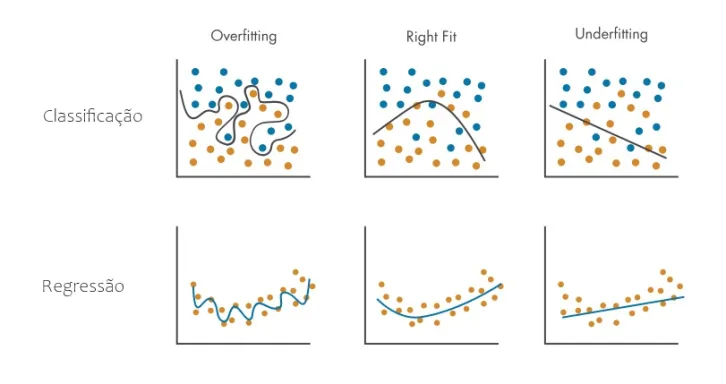
\includegraphics[width=0.8\linewidth]{img/imageoverunder.png}
    \end{figure}
\end{frame}

\begin{frame}
    \frametitle{Validação de Modelos}
    A fase de testar o nosso modelo!
    \begin{itemize}
        \item A validação de modelos avalia o desempenho de um modelo em dados não vistos durante o treinamento.
        \item Garante que o modelo generalize bem para dados do mundo real.
        \item Evita problemas como overfitting (superajuste) e underfitting (subajuste).
\end{itemize}
    
    \textbf{Técnicas comuns:}
    \begin{itemize}
            \item Divisão Treino/Validação/Teste (Hold-out)
            \item Validação Cruzada (Cross-Validation)
    \end{itemize}
\end{frame}

\begin{frame}
    \frametitle{Hold-Out}
    \begin{itemize}
        \item Divide o dataset, separando os dados para o Treinamento e para o Teste do modelo.
    \end{itemize}
    \begin{figure}
        \centering
        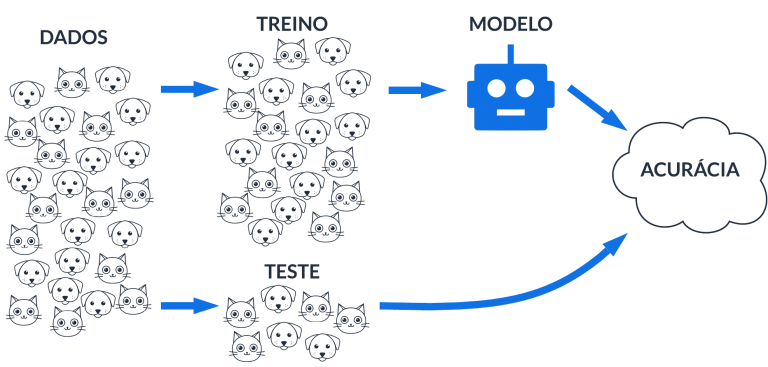
\includegraphics[width=0.8\linewidth]{img/imageholdout.png}
    \end{figure}
\end{frame}

\begin{frame}
    \frametitle{Hold-Out}
    \begin{itemize}
        \item Para modelos mais complexos os dados de treinamento são novamente divididos entre Treino e Validação, para ser possível fazer ajustes no modelo sem utilizar dos dados de Teste.
    \end{itemize}
    \begin{figure}
        \centering
        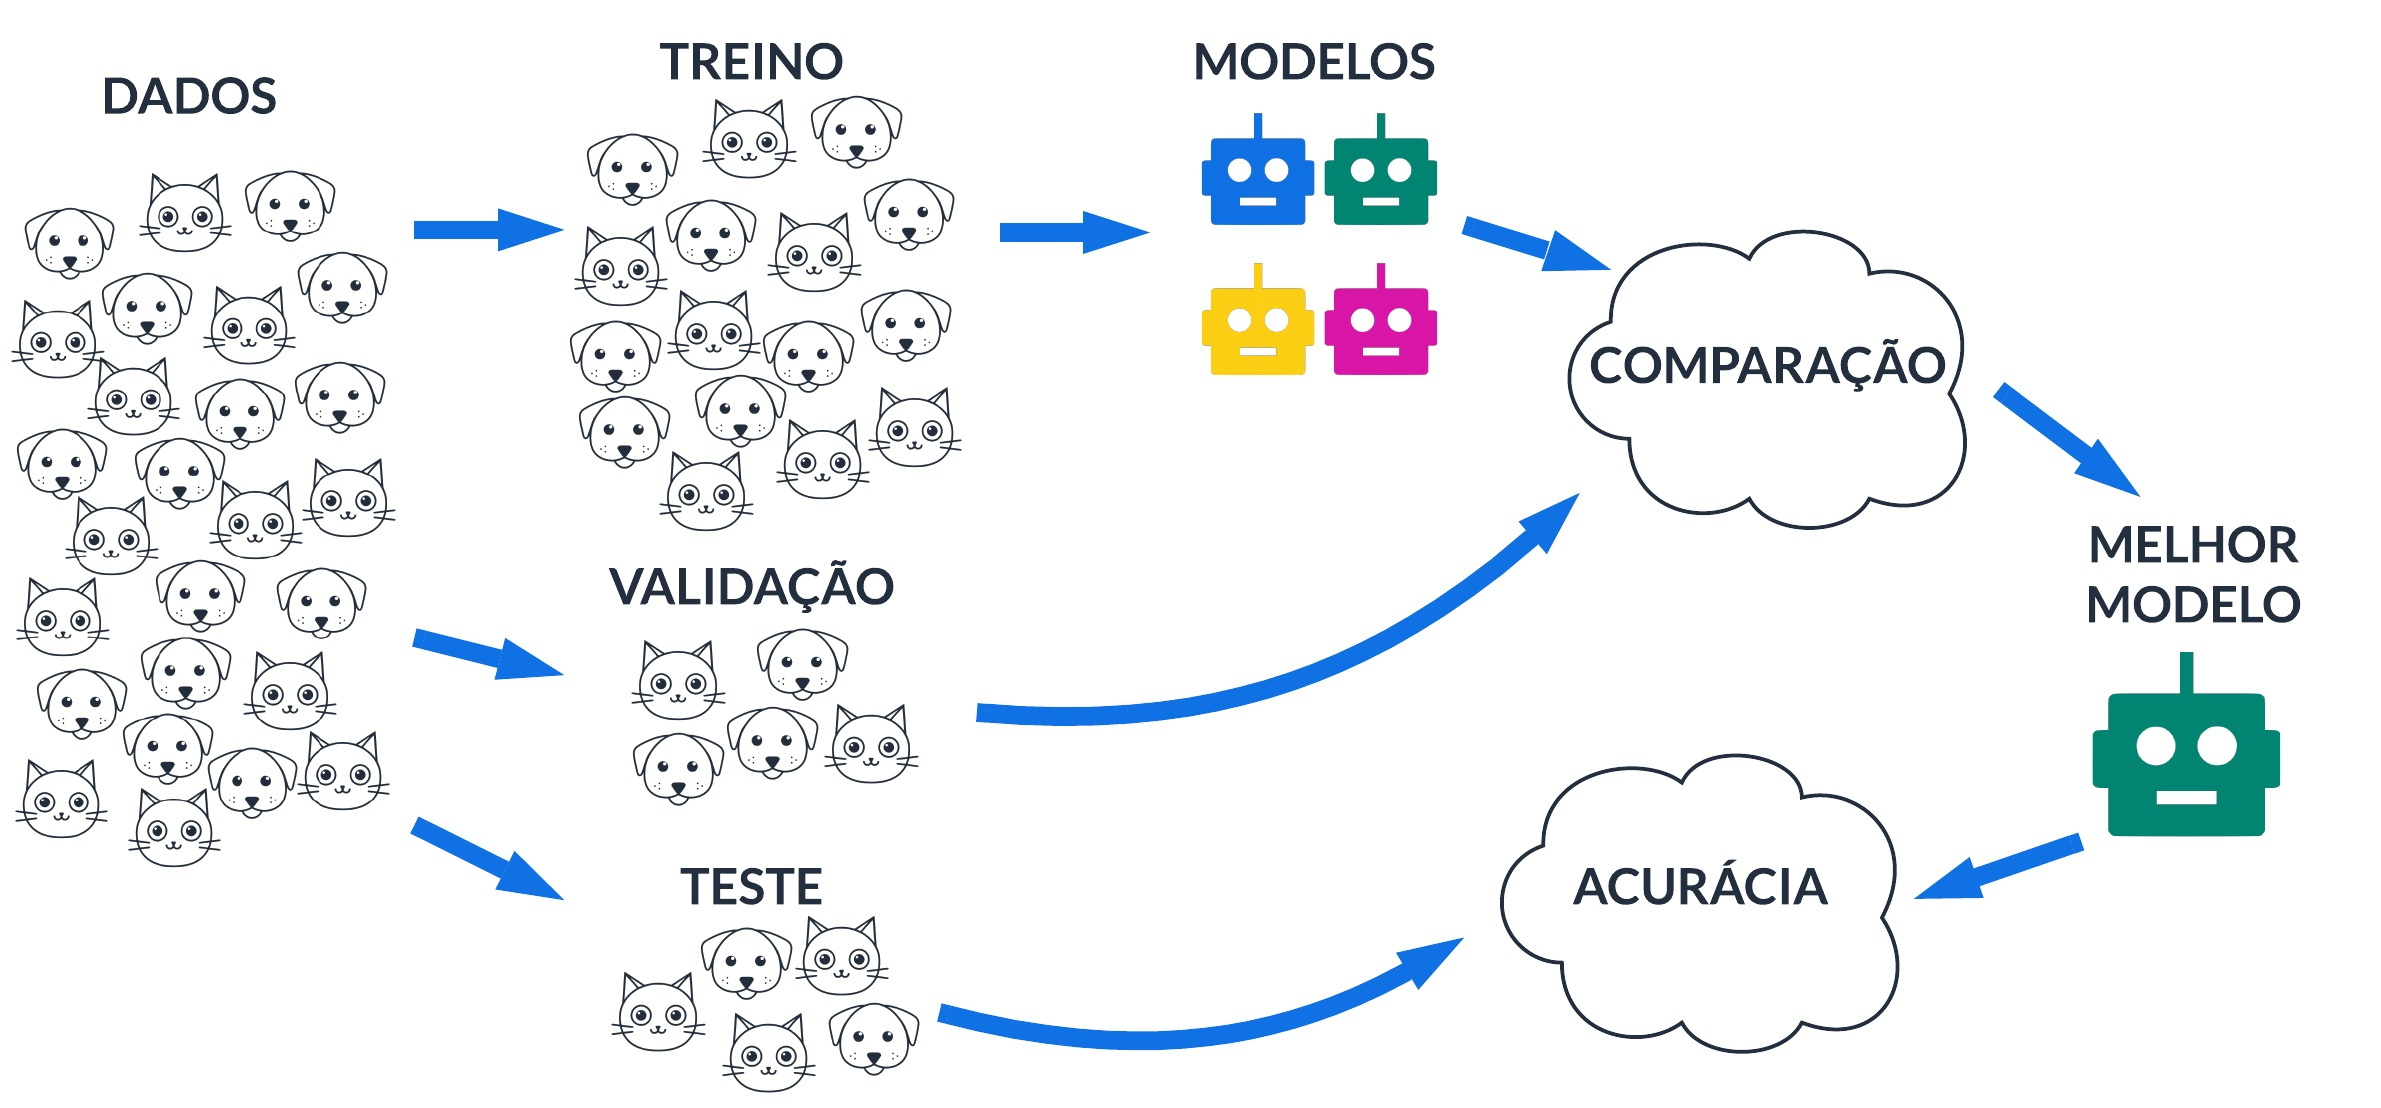
\includegraphics[width=0.8\linewidth]{img/image-ttv.png}
    \end{figure}
\end{frame}

\begin{frame}
    \frametitle{Validação Cruzada (K-fold)}
    
    \begin{itemize}
        \item Divide os dados em múltiplos subconjuntos (folds).
        \item Treina o modelo em \( k-1 \) folds e testa no fold restante.
        \item Processo repetido \( k \) vezes, garantindo que todos os dados sejam usados para treino e teste.
    \end{itemize}

    \begin{figure}
        \centering
        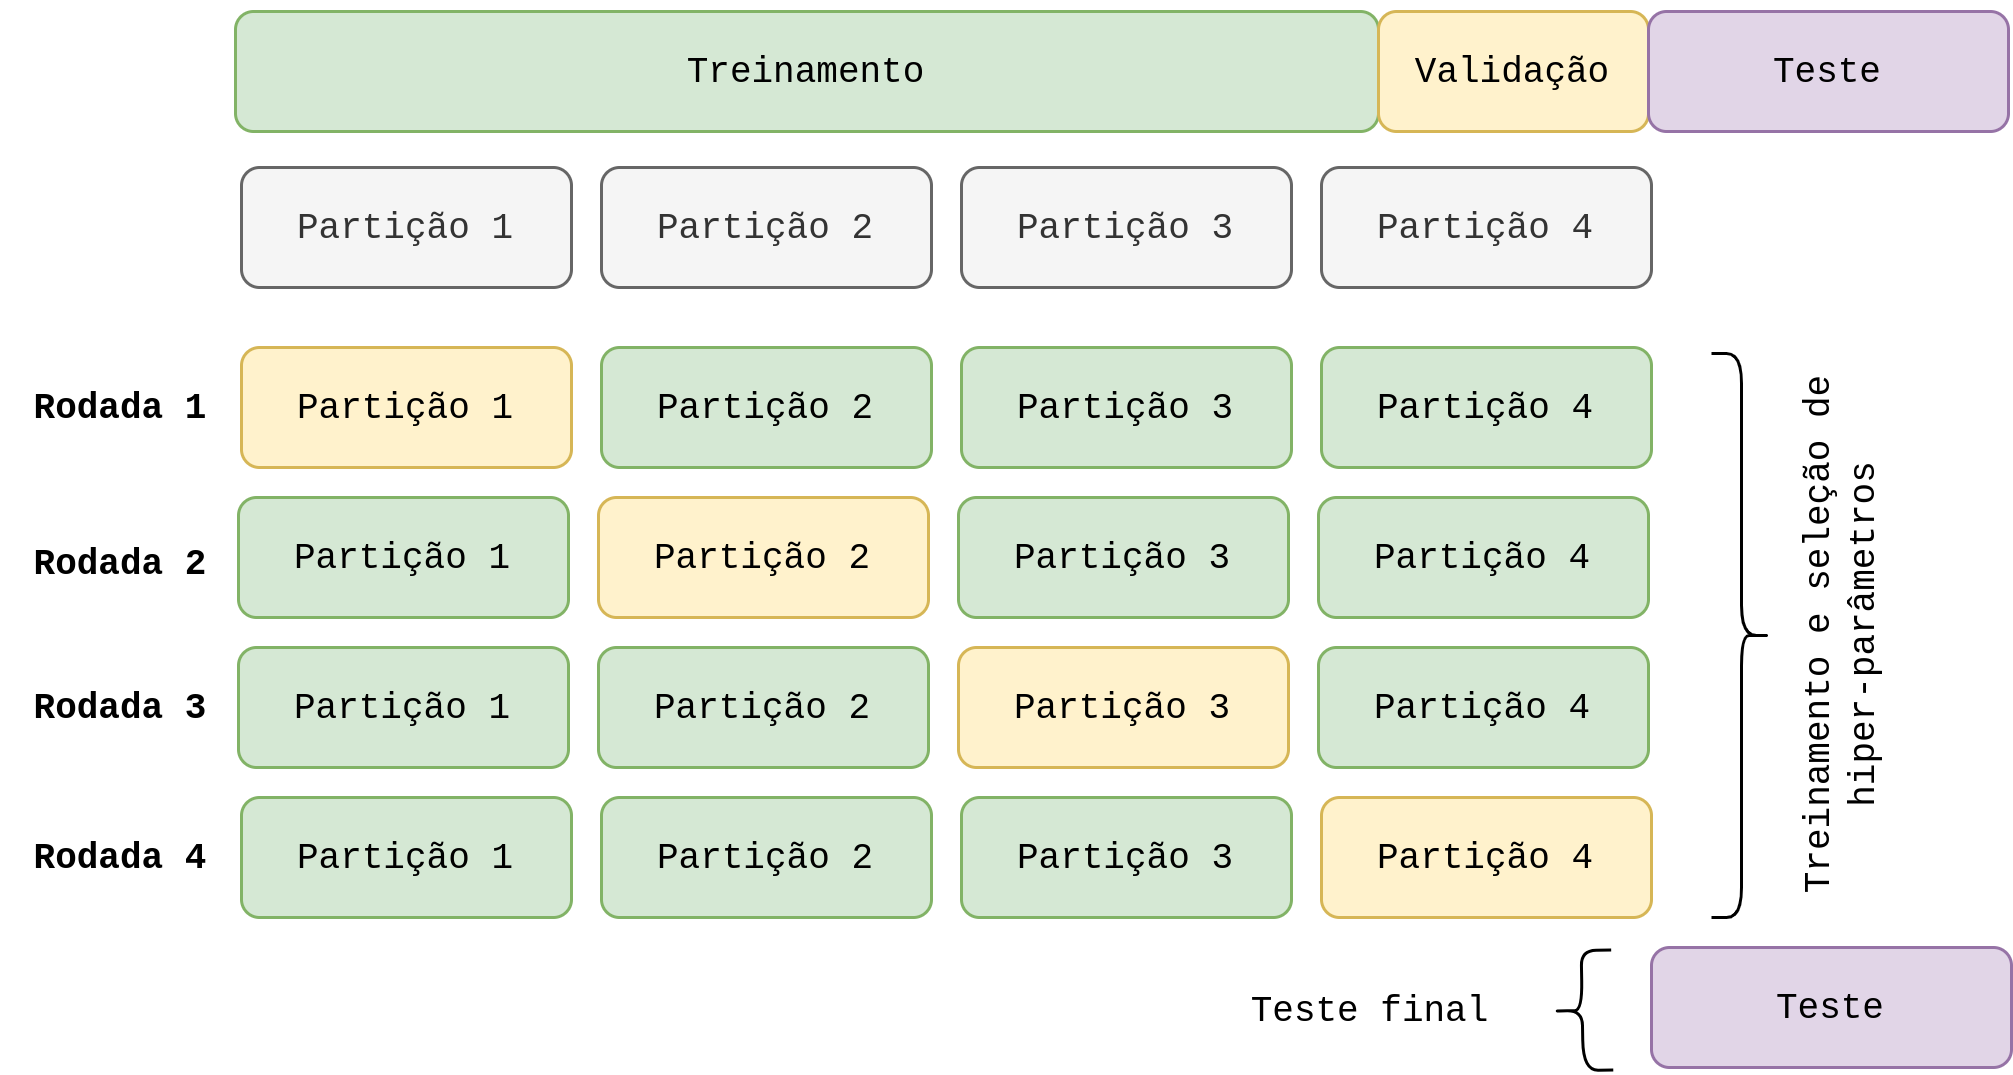
\includegraphics[width=0.7\linewidth]{img/cross_val.png}
    \end{figure}
\end{frame}